\section{Linear Regression Using Simulated Data}

For the purposes of linear regression, we write $Y_e = \a + \beta X$, although the true underlying response $Y$ will rarely be strictly deterministic and linear. It will generally include an error or residual component, in which case we write:
\begin{align}
	Y = \a + \beta X + K.
\end{align}

In the above equation, $K$ denotes the random error term, which we assume follows a normal probability distribution.

Let us simulate empirical data for $X$ and $Y$ to observe how the estimated model predictions ($Y_e$) differ from the true observed values ($Y$).

For $X$, we generate $100$ normally distributed random numbers with a theoretical mean of $1.5$ and a standard deviation of $2.5$ (though you may choose any alternate parameter pair to experiment with).

\subsection{Considerations}
\begin{enumerate}
	\item For the predicted value ($Y_e$), we assume an initial intercept $\a = 2$ and a slope $\beta = 0.3$.
	\item Subsequently, we will compute the optimal empirical estimates of $\a$ and $\beta$ using our simulated dataset to observe how the predictive efficacy of the model improves.
	\item For the actual target variable $Y$, we add a residual error term, which is simply a normally distributed random variable with mean $\mu = 0$ and standard deviation $\sigma = 0.5$.
\end{enumerate}

[,]{\texttt{fittingLinearRegression.py}}
\begin{lstlisting}[language=Python]
import pandas as pd
import numpy as np

np.random.seed(1234)

x = 2.5 * np.random.randn(100) + 1.5
res = .5 * np.random.randn(100) + 0
ypred = 2 + .3 * x
yact = 2 + .3 * x + res
xlist = x.tolist()
ypredlist = ypred.tolist()
yactlist = yact.tolist()
df = pd.DataFrame({'Input_Variable(X)': xlist, 'Predicted_Output(ypred)': ypredlist, 'Actual_Output(yact)': yactlist})
print(df.head())


import matplotlib.pyplot as plt

# x = 2.5 * np.random.randn(100) + 1.5
# res = .5 * np.random.randn(100) + 0
# ypred = 2 + .3 * x
# yact = 2 + .3 * x + res

ymean = np.mean(yact)
yavg = [ymean for i in range(1, len(xlist) + 1)]

plt.plot(x, ypred)
plt.plot(x, yact, 'ro')
plt.plot(x, yavg)
plt.title('Actual vs Predicted')
\end{lstlisting}

[,]{Screen Output}
\begin{lstlisting}[language=Python]
   Actual_Output(yact)  Input_Variable(X)  Predicted_Output(ypred)
0             2.949179           2.678588                 2.803576
1             1.840035          -1.477439                 1.556768
2             3.776326           5.081767                 3.524530
3             2.358159           0.718370                 2.215511
4             2.151703          -0.301472                 1.909558
\end{lstlisting}

\begin{center}
	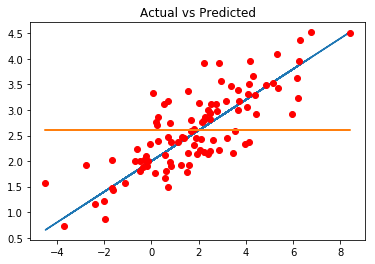
\includegraphics[width=10cm,keepaspectratio=true]{./images/actualVsPredicted.png}
\end{center}

In the preceding plot, the horizontal line represents the unconditional sample \emph{mean} of the target variable.

If we possessed no predictive regression model whatsoever, our optimal baseline prediction for any input would simply be this \emph{arithmetic mean}.

Another critical consideration is how to evaluate the predictive efficiency of our chosen model.

If you pass any historical dataset containing paired input and output variables to a statistical software package, it will mechanically compute numerical estimates for $\a$ and $\beta$.

How, then, do we ascertain whether the resulting parameters constitute a truly effective model?

\subsection{Total Sum of Squares (SST)}
\begin{align}
	SST = \sum \left( Y_i - \bar{Y} \right)^2
\end{align}
where $\bar{Y}$ represents the arithmetic mean of the actual observed values $Y_1, Y_2, \dots, Y_n$.

\subsection{Regression Sum of Squares (SSR)}
\begin{align}
	SSR = \sum \left( Y_{e,i} - \bar{Y} \right)^2
\end{align}
where $\bar{Y}$ is the average of the actual observed values, while $Y_{e,i}$ denotes the specific deterministic prediction yielded by our linear model for each observation $i$.

\subsection{Error (Residual) Sum of Squares (SSD)}
\begin{align}
	SSD = \sum \left( Y_i - Y_{e,i} \right)^2
\end{align}

Recall that $Y_e = \a + \beta X$, with $\beta$ defined by equation \eqref{beta} and $\a$ by equation \eqref{alfa}.

Using these algebraic identities, it can be proven that:
\begin{align}
	SST = SSR + SSD.
\end{align}

\begin{itemize}
	\item $SSR$: Total empirical variability explained explicitly by the linear model.
	\item $SSD$: Unexplained residual variability (model error).
	\item $SST$: Total unconditional variation in the target variable.
\end{itemize}

\begin{observacion}
	The higher the ratio of $SSR$ to $SST$, the more accurate and explanatory the regression model.
\end{observacion}

\subsection{Coefficient of Determination ($R^2$)}
\texttt{R-squared: }
\begin{align}
	R^2 = \dfrac{SSR}{SST}
\end{align}

Since $SSR \leq SST$, we must have $0 \leq R^2 \leq 1$. The closer $R^2$ approaches $1$, the superior the explanatory power of the model.

Therefore, $R^2$ serves as a reliable global indicator of whether a linear regression model is effective.

Within our Python script \texttt{fittingLinearRegression.py}, we can append the following code snippet to directly compute this $R^2$ value:

[,]{\texttt{rCuadrada.py}}
\begin{lstlisting}[language=Python]
df['SSR'] = (df['Predicted_Output(ypred)'] - ymean) ** 2
df['SST'] = (df['Actual_Output(yact)'] - ymean) ** 2
SSR = df.sum()['SSR']
SST = df.sum()['SST']
SSR / SST
\end{lstlisting}

The numerical value obtained is approximately $0.65$, which indicates a reasonably good fit. However, our assumed parameter values $\a = 2$ and $\beta = 0.3$ for $Y_e$ might not represent the absolute optimal choice.
